\chapter{Additional Design Diagrams}
\begin{figure}[H]
\centering
\begin{adjustbox}{max width=\textwidth}\begin{tikzpicture}[font=\small, >={Stealth}, st/.style={draw, rounded corners, align=center, inner sep=4pt, minimum height=0.8cm}]
  \node[st] (disc) at (0,0) {discovered};
  \node[st, right=1.4cm of disc] (wait) {waiting for\\minute 5};
  \node[st, right=1.4cm of wait] (scr) {screened\\(swaps by minute 5)};
  \node[st, right=1.4cm of scr] (scored) {scored\\(+ anatomy)};
  \node[st, below=0.9cm of scr] (not) {not scored: reason\\untradeable price $\cdot$ no trades $\cdot$ liquidity pulled\\could not read $\cdot$ missed during an outage};
  \node[st, below=0.9cm of scored] (rec) {recorded once\\(live\_prediction)};
  \node[st, right=1.2cm of rec] (res) {resolved\\6h, 1d, 7d, 30d, 90d};
  \draw[->] (disc) -- (wait); \draw[->] (wait) -- (scr); \draw[->] (scr) -- (scored);
  \draw[->] (disc) |- (not); \draw[->] (scr) -- (not); \draw[->] (wait) |- (not);
  \draw[->] (scored) -- (rec); \draw[->] (not) -- (rec); \draw[->] (rec) -- (res);
\end{tikzpicture}\end{adjustbox}
\caption{State diagram of a launch in the live scorer.}
\end{figure}
\begin{figure}[H]
\centering
\begin{adjustbox}{max width=\textwidth}\begin{tikzpicture}[font=\small, >={Stealth}, st/.style={draw, rounded corners, align=center, inner sep=4pt}]
  \node[st] (a) at (0,0) {Pool created\\(block $b$)};
  \node[st, right=1cm of a] (b) {Minute 0:\\launch type read\\(mint + LP in one tx?)};
  \node[st, right=1cm of b] (c) {Minute 5 (block $b+150$):\\features from first 5 min\\score, explain, log};
  \node[st, right=1cm of c] (d) {Hour 6:\\price ratio $\to$ buyer loss\\reserve $\to$ pulled?};
  \node[st, below=0.8cm of d] (e) {Days 1, 7, 30, 90:\\reserve $\to$ pulled?};
  \draw[->] (a) -- (b); \draw[->] (b) -- (c); \draw[->] (c) -- (d); \draw[->] (d) -- (e);
\end{tikzpicture}\end{adjustbox}
\caption{Timeline of one launch from creation to resolution.}
\end{figure}
\begin{figure}[H]\centering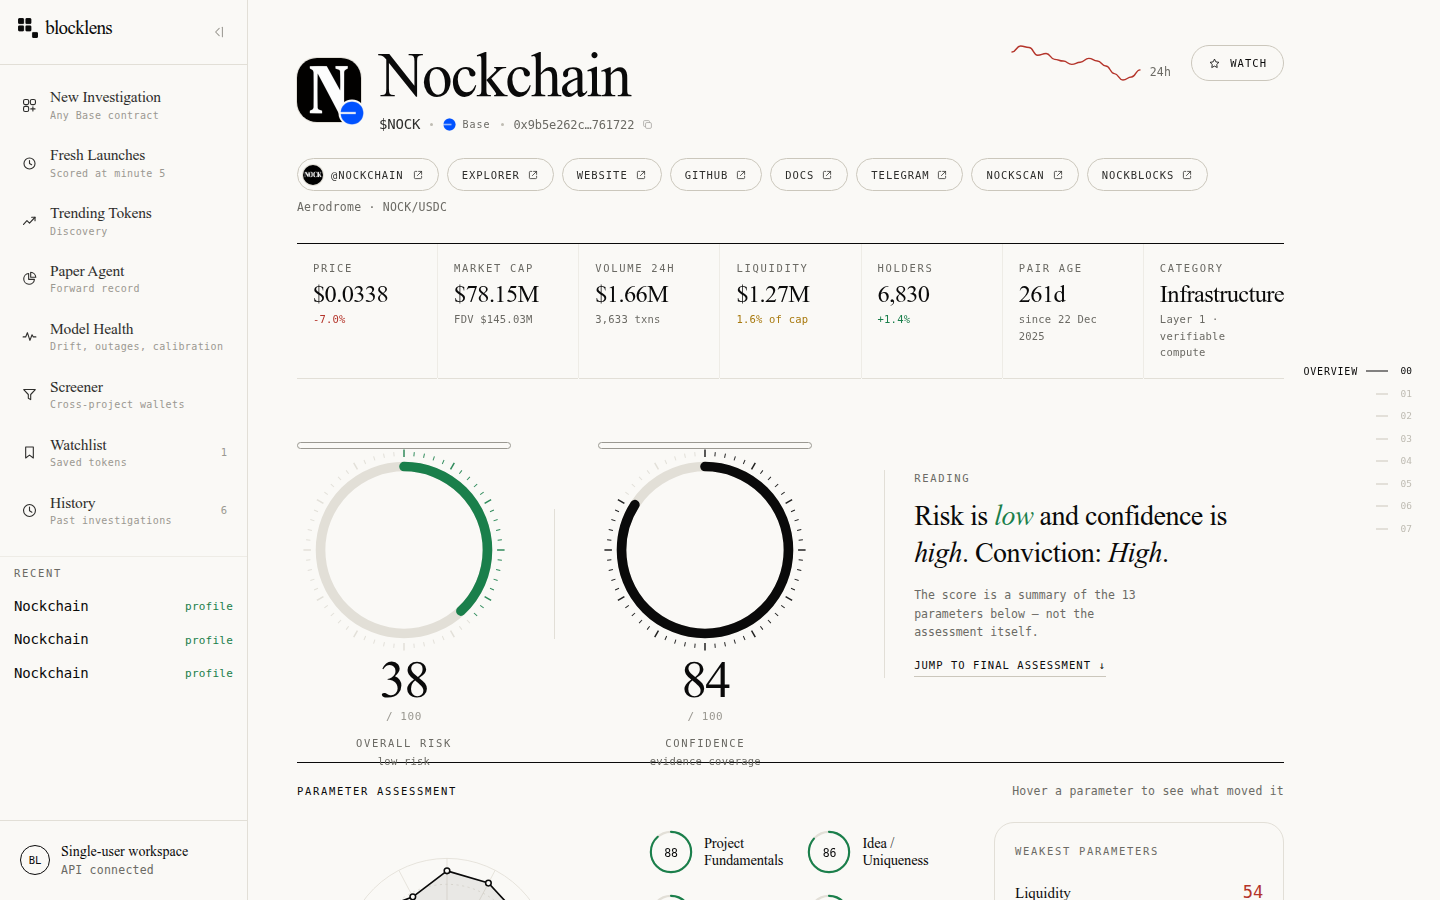
\includegraphics[width=\textwidth]{figures/profile.png}\caption{A case-study profile (Nockchain), eight sections, each marked Sourced or Sample.}\end{figure}
\begin{figure}[H]\centering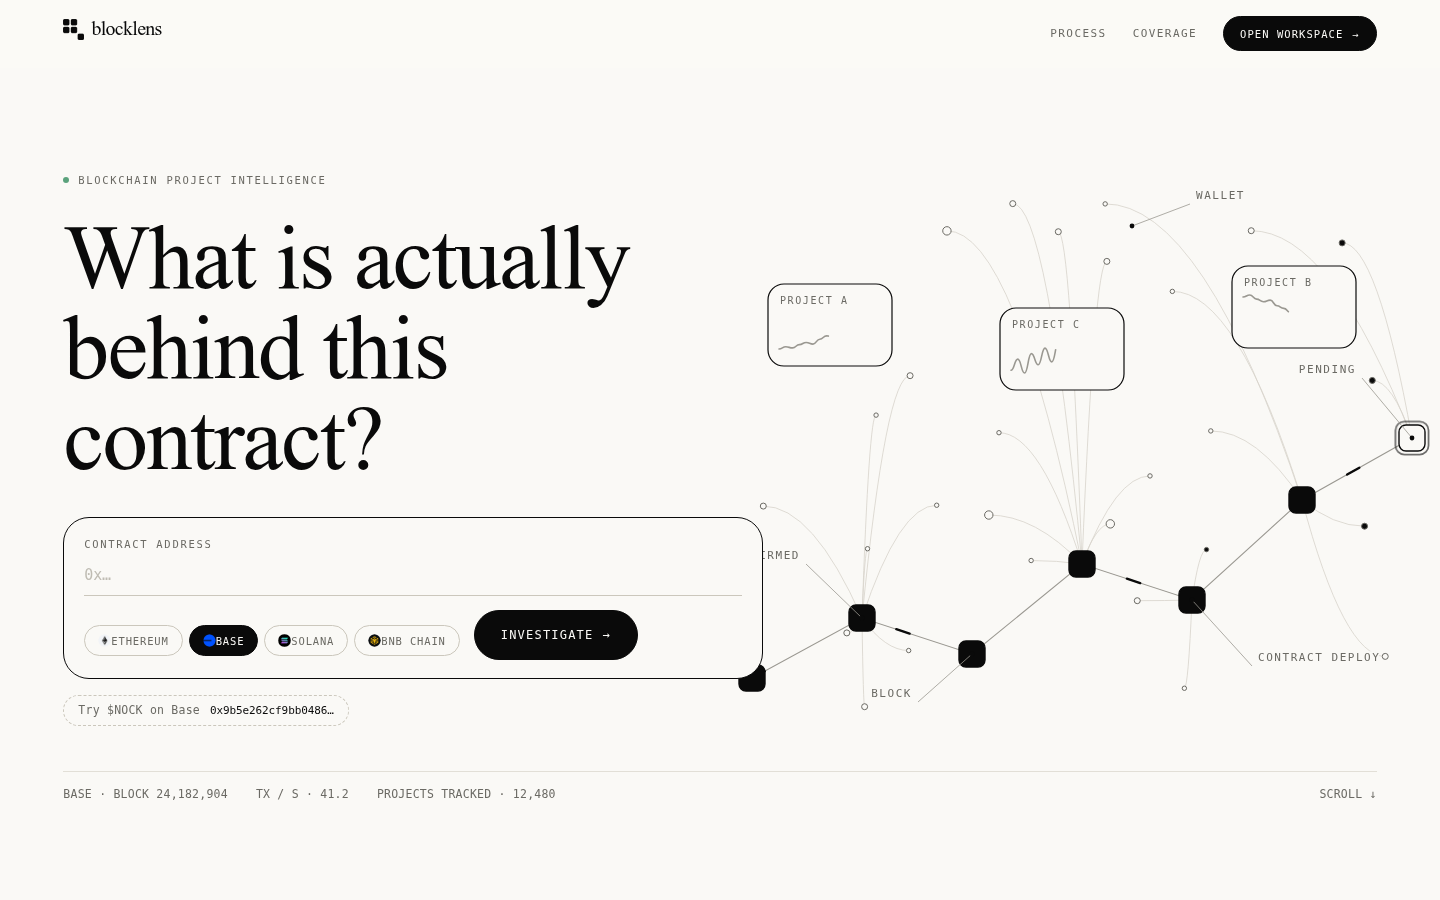
\includegraphics[width=\textwidth]{figures/landing.png}\caption{Landing page.}\end{figure}
